\graphicspath{{images/}}
\section{Результаты моделей}
Ниже приведены результаты всех моделей. Для дерева принятия решений и случайного леса сравнивается моя реализация и из библиотеки. Мягкое и жёсткое голосование использует классификаторы из предыдущей лабораторной работы.

\subsection{Дерево принятия решений}
\subsubsection{Моя реализация}
\begin{alltt}
Лучшие гиперпараметры модели: {'dtc__max_depth': 1, 'dtc__min_count': 1}
Лучший счёт модели: 0.9875
Accuracy: 0.985
Recall: 0.9726027397260274
Precision: 0.9861111111111112
\end{alltt}
\begin{center}
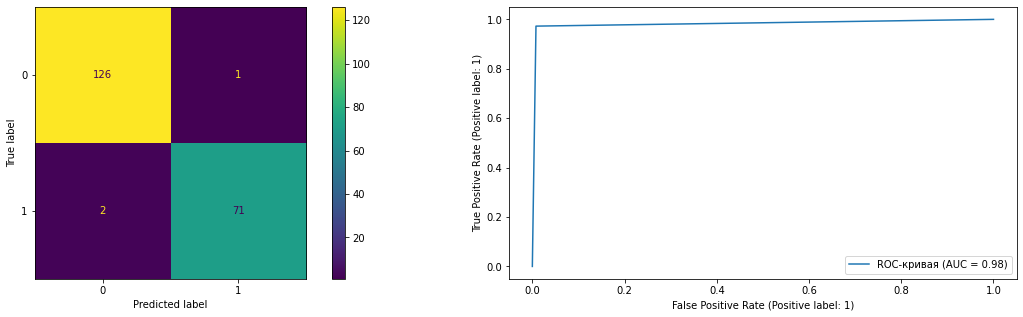
\includegraphics[width=\textwidth]{result2}
\end{center}
\pagebreak

\subsubsection{sklearn.tree.DecisionTreeClassifier}
\begin{alltt}
Лучшие гиперпараметры модели: {'dct__criterion': 'gini', 'dct__max_depth': 2, 'dct__splitter': 'best'}
Лучший счёт модели: 0.99
Accuracy: 0.99
Recall: 0.9863013698630136
Precision: 0.9863013698630136
\end{alltt}
\begin{center}
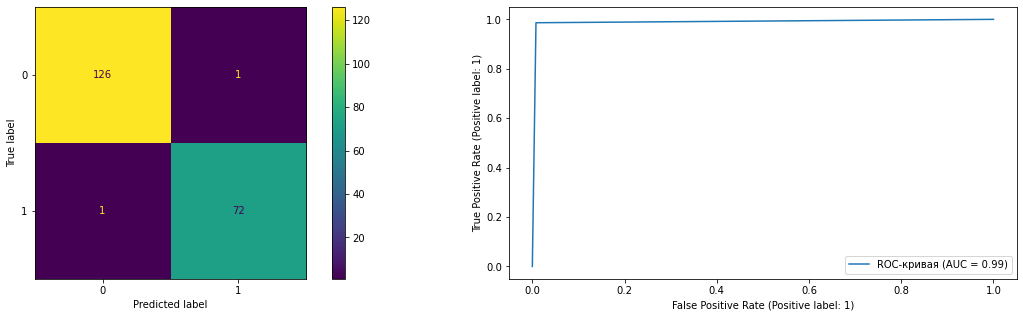
\includegraphics[width=\textwidth]{result1}
\end{center}
\pagebreak

\subsection{Случайный лес}
\subsubsection{Моя реализация}
\begin{alltt}
Лучшие гиперпараметры модели: {'rfc__max_depth': 1, 'rfc__min_count': 10, 'rfc__n_trees': 25}
Лучший счёт модели: 0.5912499999999999
Accuracy: 0.975
Recall: 0.9452054794520548
Precision: 0.9857142857142858
\end{alltt}
\begin{center}
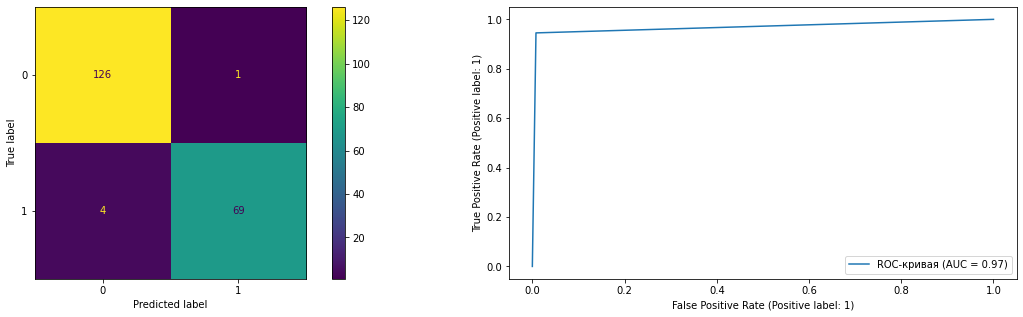
\includegraphics[width=\textwidth]{result4}
\end{center}

\subsubsection{sklearn.ensemble.RandomForestClassifier}
\begin{alltt}
Лучшие гиперпараметры модели: {'dct__criterion': 'log_loss', 'dct__max_depth': 4, 'dct__n_estimators': 25}
Лучший счёт модели: 0.9950000000000001
Accuracy: 0.99
Recall: 0.9863013698630136
Precision: 0.9863013698630136
\end{alltt}
\begin{center}
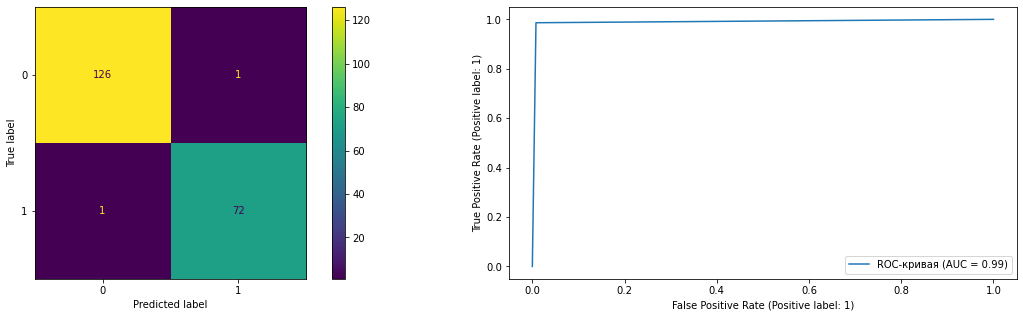
\includegraphics[width=\textwidth]{result1}
\end{center}
\pagebreak

\subsection{Градиентный бустинг}
\subsubsection{sklearn.ensemble.GradientBoostingClassifier}
\begin{alltt}
Лучшие гиперпараметры модели: {'gbc__learning_rate': 0.01, 'gbc__n_estimators': 50}
Лучший счёт модели: 0.99125
Accuracy: 0.99
Recall: 0.9863013698630136
Precision: 0.9863013698630136
\end{alltt}
\begin{center}
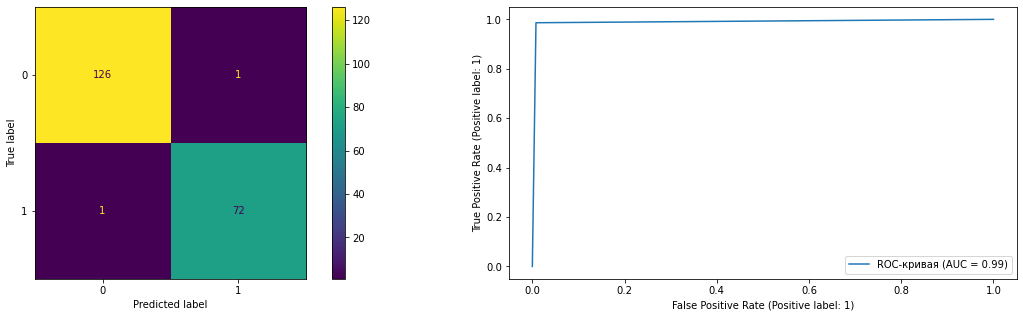
\includegraphics[width=\textwidth]{result1}
\end{center}

\subsection{Мягкое и жёсткое голосование}
Для голосования используются одни и те же модели:
\begin{lstlisting}[language=Python]
models = []
models.append(kNN_p(3))
models.append(LogisticRegression_p(SGD_step = 0.05, batch_size = 5, epoches = 2))
models.append(SVM_p(SGD_step =  0.01, alpha = 1.0, batch_size = 5, epoches = 4))
models.append(NaiveBayes_p())
models.append(MyDecisionTreeClassifier_p(max_depth = 2, min_count = 5))
\end{lstlisting}
\pagebreak

\subsubsection{Мягкое голосование}
\begin{alltt}
Accuracy: 0.985
Recall: 0.9726027397260274
Precision: 0.9861111111111112
\end{alltt}
\begin{center}
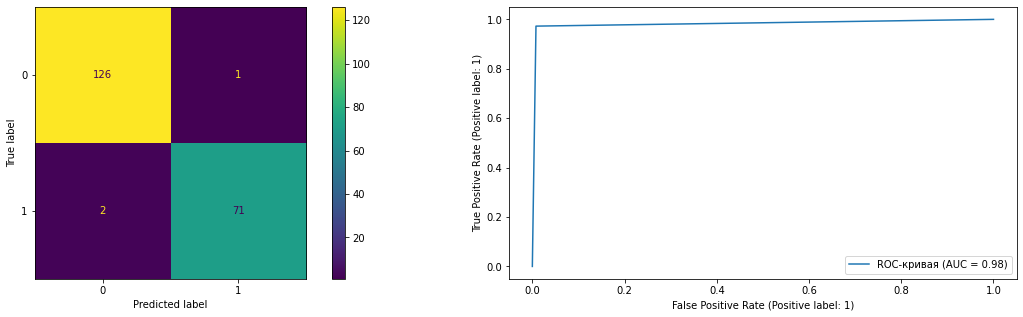
\includegraphics[width=\textwidth]{result2}
\end{center}

\subsubsection{Жёсткое голосование}
\begin{alltt}
Accuracy: 0.99
Recall: 0.9863013698630136
Precision: 0.9863013698630136
\end{alltt}
\begin{center}
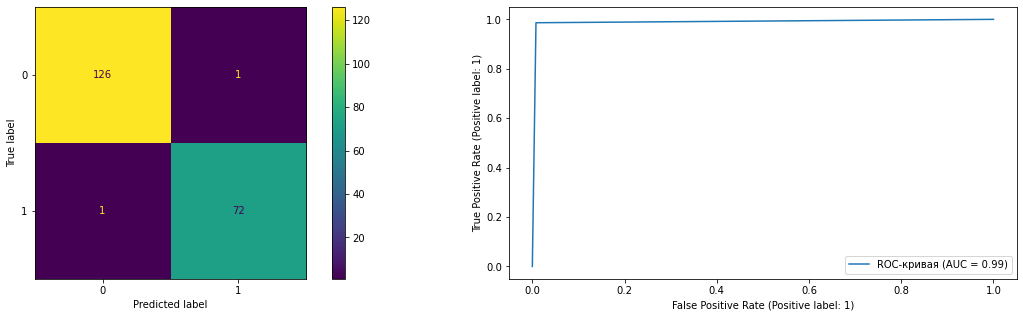
\includegraphics[width=\textwidth]{result1}
\end{center}
\pagebreak

\pagebreak
